\chapter{Lạm phát từ một trường vô hướng đang lăn}

\lectureoverview{Một câu hỏi còn lại từ buổi trước cung cấp phương trình chủ đạo,
\(\ddot\phi+3H\dot\phi=-V'(\phi)\): cái gì chuyển động, cái gì tác dụng lực, và vì sao sự giãn nở lại giống ma sát? Trước hết chúng ta suy ra phương trình đó trong một hộp cố định rồi sau đó trong một hộp đang giãn nở. Ghép nó với phương trình Friedmann cho ta cơ chế lăn chậm, trong đó một thế vô hướng cao và thoải điều khiển sự giãn nở gần như hàm mũ. Lạm phát làm loãng các đơn cực và làm trơn hình học; khi kết thúc, nó nung nóng lại vũ trụ và mở đầu Vụ Nổ Lớn nóng thông thường. Khi đó bài toán cuối cùng trở nên không thể tránh khỏi: nếu lạm phát làm trơn hiệu quả đến vậy, cấu trúc từ đâu mà có? Một phép tính caustic một chiều cho thấy những biến thiên rất nhỏ của vận tốc tạo ra các tấm, sợi và nút như thế nào, đồng thời dời nguồn gốc lượng tử của những biến thiên đó sang bài giảng tiếp theo.}

\section{Cái gì tác dụng lên cái gì?}

Câu hỏi mở đầu nhắc lại phương trình
\begin{equation}
\ddot\phi+3H\dot\phi
=F(\phi)
=-\frac{dV}{d\phi}
\label{eq:c09-opening}
\end{equation}
và hỏi loại lực nào \(F\) có thể tác dụng lên một trường. Câu hỏi đó không hề thứ yếu. Để trả lời, ta phải dựng lại cơ học của trường, và qua đó mở đầu cho chính chủ đề lạm phát.

Một trường vô hướng gán một số \(\phi(\mathbf x,t)\) cho mỗi điểm trong không gian và thời gian. Điện trường và từ trường mang năng lượng; trường vô hướng cũng có thể mang năng lượng. Trường cần ở đây là giả thuyết: chưa có inflaton cụ thể nào được nhận diện bằng thực nghiệm, nên chưa biết năng lượng của nó như một hàm của giá trị trường. Vì vậy ta biểu diễn nó bằng một mật độ thế năng chưa xác định
\begin{equation}
V=V(\phi).
\label{eq:c09-potential}
\end{equation}
Các giá trị khác nhau của \(\phi\) tương ứng với những lượng năng lượng khác nhau được tích trữ trên mỗi đơn vị thể tích vật lý.

Không có lý do gì để \(\phi=0\) có năng lượng bằng không. Gốc của không gian trường chỉ là một quy ước, đặc biệt đối với một trường chưa được phát hiện, và việc tịnh tiến tọa độ dùng để gắn nhãn các giá trị trường không nhất thiết đặt cực tiểu của \(V\) tại gốc. Đồ thị của \(V(\phi)\) mô tả các độ dốc và độ cao tương đối, chứ không phải một điểm xuất phát đặc quyền cho trường.

Thế năng là phần còn lại khi trường tức thời đứng yên. Nếu trường biến thiên theo thời gian thì nó còn có động năng. Đại lượng \(\dot\phi\) không phải vận tốc của một vật chuyển động qua không gian thông thường; nó là tốc độ thay đổi của giá trị trường, tức một vận tốc trong không gian trường. Một sợi dây đàn hồi là phép loại suy hữu ích. Độ dời của nó là một trường trên một thế giới một chiều, và một phần tử dây đang dao động mang động năng tỉ lệ với bình phương đạo hàm theo thời gian của nó.

Hệ số của bình phương đó có thể được hấp thụ vào định nghĩa của trường. Nếu bắt đầu với
\begin{equation}
\frac12 n^2\dot\phi^{\,2},
\end{equation}
thì phép đổi biến
\begin{equation}
\chi=n\phi
\end{equation}
biến số hạng đó thành \(\dot\chi^{\,2}/2\). Vì vậy ta có thể chọn một trường được chuẩn hóa chính tắc và viết, trong gần đúng đồng nhất,
\begin{equation}
\rho_\phi=\frac12\dot\phi^{\,2}+V(\phi).
\label{eq:c09-rho-homogeneous}
\end{equation}
Lựa chọn này là sự chuẩn hóa của tọa độ trong không gian trường, chứ không phải khẳng định rằng một khối lượng hạt theo nghĩa đen đã được đặt bằng một.

\section{Cơ học trong một hộp cố định}

Xét một hộp nhỏ mà trong đó trường gần như không đổi theo không gian. Mật độ năng lượng của nó có cùng dạng toán học như năng lượng của một hạt khối lượng đơn vị: động năng cộng thế năng. Mật độ Lagrange tương ứng có dấu ngược đối với thế năng,
\begin{equation}
\mathcal L_\phi
=\frac12\dot\phi^{\,2}-V(\phi).
\label{eq:c09-lagrangian-density}
\end{equation}
Phép tương tự này là về mặt toán học. Tọa độ suy rộng là giá trị của trường, không phải vị trí không gian của một hạt.

Phương trình Euler--Lagrange là
\begin{equation}
\frac{d}{dt}
\left(
\frac{\partial\mathcal L_\phi}{\partial\dot\phi}
\right)
=
\frac{\partial\mathcal L_\phi}{\partial\phi}.
\label{eq:c09-el-fixed}
\end{equation}
Ở đây biến vận tốc là \(\dot\phi\), nên
\begin{equation}
\frac{\partial\mathcal L_\phi}{\partial\dot\phi}=\dot\phi,
\qquad
\frac{\partial\mathcal L_\phi}{\partial\phi}=-V'(\phi),
\end{equation}
ta thu được
\begin{equation}
\ddot\phi=-V'(\phi)\equiv F(\phi).
\label{eq:c09-fixed-eom}
\end{equation}
Đạo hàm bậc hai là gia tốc của tọa độ trường, còn độ dốc âm của thế năng là lực của nó.

\begin{figure}[htbp]
\centering
\includegraphics[width=0.88\textwidth]{lecture_09_figure_03.png}
\caption{Phần đọc được trên bảng nối \(V(\phi)\) với phương trình hộp cố định \(\ddot\phi=-\partial V/\partial\phi\). Biểu thức Euler--Lagrange ở phía trên bị cắt bớt và che khuất một phần, nên phương trình~\eqref{eq:c09-el-fixed} được phục dựng từ phép suy ra chứ không được trích như một bản chép trọn vẹn của khung hình.}
\label{fig:c09-fixed-board}
\lectureframe{00:10:53.836}
\end{figure}

\begin{classroomqa}
\audiencequestion{Lực là gì, và nó tác dụng lên cái gì?}
\lecturerresponse{Đại lượng đang biến đổi là giá trị vô hướng \(\phi\). Đại lượng \(-V'(\phi)\) là một lực trong không gian trường: nó gia tốc giá trị trường về phía thế năng thấp hơn, đúng như \(-dV/dx\) gia tốc một tọa độ hạt. Nó không phải là một lực vectơ mới đẩy một vật thể vật chất đi qua không gian thông thường. \lecturetimestamp{00:00:27--00:00:49; 00:10:41--00:11:29}}
\end{classroomqa}

Trường đầy đủ có thể phụ thuộc vào không gian. Đối với một vô hướng chính tắc trong một hình học giãn nở phẳng theo không gian, mật độ năng lượng cục bộ của nó chứa
\begin{equation}
\rho_\phi
=
\frac12\dot\phi^{\,2}
+\frac{1}{2a^2}\lvert\nabla\phi\rvert^2
+V(\phi).
\label{eq:c09-rho-full}
\end{equation}
Ta bỏ số hạng gradient vì sự giãn nở kéo dãn các biến thiên tới bước sóng dài, khiến trường gần như đồng nhất bên trong hộp nhỏ. Đây là một gần đúng được bối cảnh vũ trụ học biện minh, chứ không phải sự phủ nhận rằng sóng vô hướng hay các gợn theo không gian có thể tồn tại.

\section{Hộp đang giãn nở}

Phép suy ra thứ nhất trả lời câu hỏi mở đầu, nhưng đó vẫn chưa phải là phép suy ra vũ trụ học. Các phương trình~\eqref{eq:c09-rho-homogeneous} và \eqref{eq:c09-lagrangian-density} là các mật độ. Một hộp đồng chuyển động đơn vị có thể tích vật lý tỉ lệ với \(a^3(t)\), nên Lagrangian của nó là
\begin{equation}
L_\phi
=a^3(t)
\left[
\frac12\dot\phi^{\,2}-V(\phi)
\right].
\label{eq:c09-comoving-lagrangian}
\end{equation}
Hệ số \(a^3\) sẽ không quan trọng trong một hộp tĩnh. Trong vũ trụ học nó phụ thuộc vào thời gian, và sự phụ thuộc đó cung cấp số hạng còn thiếu.

\begin{figure}[htbp]
\centering
\includegraphics[width=0.88\textwidth]{lecture_09_figure_04.png}
\caption{Một đường cong thế năng vẽ tay hiện rõ ở bên trái, còn ở bên phải xuất hiện các mảnh của những biểu thức năng lượng và Lagrangian. Đường cong và sự đổi dấu là chắc chắn; toàn bộ phép biến đổi đại số trong phương trình~\eqref{eq:c09-comoving-lagrangian} được lấy từ phần suy ra bằng lời vì giảng viên che khuất một phần của bảng.}
\label{fig:c09-potential-board}
\lectureframe{00:13:26.528}
\end{figure}

Áp dụng phương trình Euler--Lagrange cho \(L_\phi\) cho
\begin{align}
\frac{d}{dt}\left(a^3\dot\phi\right)
&=-a^3V'(\phi), \label{eq:c09-a3-form}\\
a^3\ddot\phi+3a^2\dot a\,\dot\phi
&=-a^3V'(\phi),\\
\ddot\phi+3\frac{\dot a}{a}\dot\phi
&=-V'(\phi).
\end{align}
Với \(H=\dot a/a\), ta được
\begin{equation}
\boxed{\ddot\phi+3H\dot\phi=-V'(\phi)}.
\label{eq:c09-hubble-friction}
\end{equation}
Phương trình được nhớ lại ở phần đầu nay đã được suy ra chứ không chỉ đơn thuần được nhắc lại.

\begin{figure}[htbp]
\centering
\includegraphics[width=0.96\textwidth]{lecture_09_figure_05.png}
\caption{Động lực học của hộp cố định ở bên trái và hiệu chỉnh do hộp giãn nở ở bên phải. Phần bảng còn nhìn thấy được cho thấy chuỗi từ \(d(a^3\dot\phi)/dt\) tới các dạng \(3\dot a/a\) và \(3H\); các vế phải bị cắt được cung cấp bởi phương trình~\eqref{eq:c09-a3-form}.}
\label{fig:c09-expanding-board}
\lectureframe{00:18:35.380}
\end{figure}

\begin{classroomqa}
\audiencequestion{Có thể hình dung lực \(F\) một cách cụ thể hơn không?}
\lecturerresponse{Hãy vẽ \(V(\phi)\) như một địa hình mà tọa độ ngang là giá trị của trường. Độ dốc xác định lực, \(F=-V'(\phi)\). Một sườn dốc đi xuống lớn tạo ra sự thúc đẩy mạnh trong không gian trường; một sườn dốc thoải tạo ra sự thúc đẩy yếu. Hình ảnh này là công cụ hỗ trợ cho tọa độ trường một chiều, không phải một ngọn đồi thật sự nằm trong không gian vật lý. \lecturetimestamp{00:18:26--00:19:18}}
\end{classroomqa}

\section{Ma sát Hubble và chuyển động tới vận tốc giới hạn}

Chuyển số hạng ở giữa trong phương trình~\eqref{eq:c09-hubble-friction} sang vế phải:
\begin{equation}
\ddot\phi=-V'(\phi)-3H\dot\phi.
\end{equation}
Đối với một vũ trụ đang giãn nở \(H>0\), số hạng thứ hai luôn chống lại vận tốc của trường. Vì thế nó ứng xử như độ nhớt. Một hòn đá thả vào mật ong đặc ban đầu gia tốc, nhưng lực cản tăng theo tốc độ cho đến khi hòn đá đạt vận tốc giới hạn. Mẹo ghi nhớ \emph{\(H\) ứng với mật ong} nắm bắt phép tương tự này, còn phương trình cho nội dung thực sự của nó. Nếu \(H\) thay đổi theo thời gian vũ trụ, thì độ nhớt hiệu dụng cũng thay đổi, cũng như độ nhớt thông thường thay đổi theo nhiệt độ.

Khi ma sát chi phối quán tính, \(\lvert\ddot\phi\rvert\ll3H\lvert\dot\phi\rvert\), trường nhanh chóng tiến tới
\begin{equation}
3H\dot\phi\simeq -V'(\phi),
\qquad
\dot\phi\simeq-\frac{V'(\phi)}{3H}.
\label{eq:c09-terminal}
\end{equation}
Một thế năng thoải cung cấp một lực nhỏ, còn một \(H\) lớn cung cấp lực cản mạnh. Cả hai hiệu ứng đều làm \(\dot\phi\) nhỏ và thường làm cho mật độ động năng \(\dot\phi^2/2\) nhỏ so với \(V\).

\begin{classroomqa}
\audiencequestion{Phép suy ra này có dựa vào nguyên lý tác dụng tối thiểu không?}
\lecturerresponse{Có. Phương trình~\eqref{eq:c09-hubble-friction} thu được bằng cách cực trị hóa tác dụng xây dựng từ phương trình~\eqref{eq:c09-comoving-lagrangian}. Ta cũng có thể lấy phương trình trường làm định luật động lực học khởi đầu, nhưng phép suy ra biến phân giải thích chính xác vì sao thể tích đang giãn nở lại đóng góp \(3H\dot\phi\). \lecturetimestamp{00:25:40--00:26:15}}
\end{classroomqa}

\begin{classroomqa}
\audiencequestion{Nếu số hạng mới tác dụng như ma sát, năng lượng bị mất đi sẽ đi đâu?}
\lecturerresponse{Một hòn đá thật trong mật ong truyền năng lượng cơ học thành nhiệt. Phát biểu vũ trụ học thì tinh tế hơn. Lagrangian của hộp đồng chuyển động phụ thuộc tường minh vào thời gian thông qua \(a(t)\), nên năng lượng cơ học thông thường của hộp đó không được bảo toàn bởi đối xứng tịnh tiến theo thời gian. Bảo toàn hiệp biến cục bộ của năng lượng-động lượng vẫn đúng:
\[
\dot\rho_\phi+3H(\rho_\phi+p_\phi)=0,
\qquad
p_\phi=\frac12\dot\phi^{\,2}-V(\phi).
\]
Đối với một vô hướng đồng nhất, điều này trở thành \(\dot\rho_\phi=-3H\dot\phi^{\,2}\): trường thực hiện công lên hình học đang giãn nở. Điều không còn đúng là một năng lượng toàn cục được bảo toàn theo nghĩa ngây thơ cho vũ trụ đang tiến hóa, chứ không phải bảo toàn cục bộ của năng lượng-động lượng. \lecturetimestamp{00:26:16--00:27:57}}
\end{classroomqa}

\section{Trường thúc đẩy sự giãn nở}

Cho đến đây, sự giãn nở đã tác động lên trường vô hướng. Đó mới chỉ là một nửa của vòng phản hồi. Mật độ năng lượng của trường vô hướng cũng quyết định sự giãn nở thông qua phương trình Friedmann cho không gian phẳng,
\begin{equation}
H^2=\left(\frac{\dot a}{a}\right)^2
=\frac{8\pi G}{3}\rho.
\label{eq:c09-friedmann}
\end{equation}
Đối với một trường vô hướng gần như đồng nhất,
\begin{equation}
H^2
=\frac{8\pi G}{3}
\left[
\frac12\dot\phi^{\,2}+V(\phi)
\right].
\label{eq:c09-friedmann-scalar}
\end{equation}
Sự giãn nở làm hãm trường, và trường bị hãm đó đến lượt nó có thể duy trì mật độ năng lượng thúc đẩy sự giãn nở.

\begin{classroomqa}
\audiencequestion{Trường vô hướng giả định này có phải là cái người ta gọi là inflaton không?}
\lecturerresponse{Đúng. Tên gọi này mô tả vai trò người ta gán cho nó: một trường vô hướng có thế năng gần như không đổi thúc đẩy lạm phát. Việc đặt tên cho trường không xác định vật lý hạt của nó. Inflaton cụ thể, các ghép cặp của nó, và thậm chí liệu chỉ một trường vô hướng sơ cấp duy nhất có đảm nhiệm vai trò này hay không, vẫn còn phụ thuộc mô hình. \lecturetimestamp{00:30:26--00:31:28}}
\end{classroomqa}

\begin{classroomqa}
\audiencequestion{Có bằng chứng thực nghiệm nào cho inflaton không?}
\lecturerresponse{Không có phát hiện trực tiếp nào trong phòng thí nghiệm về một trường inflaton cụ thể. Bằng chứng là gián tiếp: động lực học lạm phát cung cấp một khuôn khổ thành công cho độ phẳng quan sát được và các nhiễu loạn nguyên thủy, nhưng nhiều thế năng có thể phù hợp với những dữ kiện khái quát đó. Cần tách sự hậu thuẫn gián tiếp này khỏi hiểu biết về sự hiện thực hóa vi mô. \lecturetimestamp{00:31:29--00:33:02}}
\end{classroomqa}

\begin{classroomqa}
\audiencequestion{Mọi trường đều mang năng lượng, và một kích thích vô hướng có phải là boson không?}
\lecturerresponse{Các trường vật lý đóng góp năng lượng và xung lượng. Việc lượng tử hóa một trường vô hướng sinh ra các lượng tử boson spin-0. Nền đồng nhất cổ điển dùng trong lạm phát không nên được hình dung như một hạt thông thường đơn lẻ, mặc dù sau lạm phát các dao động của nó có thể được mô tả theo các lượng tử inflaton. \lecturetimestamp{00:33:03--00:35:20}}
\end{classroomqa}

\begin{classroomqa}
\audiencequestion{Liệu trường Higgs có thể là inflaton không?}
\lecturerresponse{Cần một trường vô hướng, nên sự tương tự này là tự nhiên, nhưng Higgs đã được quan sát, với thế năng và các ghép cặp Mô hình Chuẩn thông thường của nó, không tự động là trường được mô tả bởi cao nguyên đơn giản này. Các mô hình lạm phát Higgs bổ sung cấu trúc hấp dẫn phi tối thiểu. Không có gì trong lập luận hiện tại xác định inflaton là Higgs. \lecturetimestamp{00:35:21--00:37:11}}
\end{classroomqa}

Bây giờ hãy hình dung \(V(\phi)\) có giá trị cao nhưng dốc thoai thoải trên một khoảng dài. Phương trình~\eqref{eq:c09-terminal} giữ cho trường chuyển động chậm, và do đó
\begin{equation}
\frac12\dot\phi^{\,2}\ll V(\phi).
\end{equation}
Phương trình Friedmann rút gọn thành
\begin{equation}
H^2\simeq\frac{8\pi G}{3}V(\phi),
\qquad
H\simeq
\sqrt{\frac{8\pi G}{3}V(\phi)}.
\label{eq:c09-potential-dominated}
\end{equation}
Đạo hàm \(V'(\phi)\) chi phối chuyển động chậm của trường; độ cao \(V(\phi)\) chi phối sự giãn nở nhanh của không gian.

\begin{figure}[htbp]
\centering
\includegraphics[width=0.92\textwidth]{lecture_09_figure_06.png}
\caption{Phương trình Friedmann, mật độ năng lượng của trường vô hướng, và biểu thức bị thế năng chi phối được đóng khung. Hạng căn bậc hai trong \(V(\phi)\) là rõ ràng; cụm mở đầu \(H\simeq\) trong phương trình~\eqref{eq:c09-potential-dominated} là phần hoàn thiện chuẩn, đúng như lập luận bằng lời đã nêu.}
\label{fig:c09-friedmann-board}
\lectureframe{00:41:04.178}
\end{figure}

Nếu \(V\) chỉ thay đổi rất ít khi trường đi qua cao nguyên, thì \(H\) gần như không đổi. Lấy tích phân \(\dot a/a\simeq H\) cho
\begin{equation}
a(t)\simeq a_i e^{H(t-t_i)}.
\label{eq:c09-exponential}
\end{equation}
Đây là lạm phát. Thời gian tăng gấp đôi trong vũ trụ sơ khai cỡ \(10^{-32}\,\mathrm{s}\) cho thấy tính dữ dội của nó; con số này chỉ có tính minh họa và phụ thuộc vào thang năng lượng lạm phát.

\begin{classroomqa}
\audiencequestion{Làm thế nào một trường chuyển động chậm lại có thể tạo ra một vũ trụ giãn nở nhanh?}
\lecturerresponse{Chuyển động chậm là \(\phi\), chứ không phải \(a\). Ma sát Hubble ngăn trường lao nhanh xuống thế năng, nên \(V(\phi)\) gần như không đổi. Một \(V\) lớn và gần như không đổi cho một \(H\) lớn và gần như không đổi, và khi đó hệ số tỉ lệ tăng theo hàm mũ. Độ dốc nhỏ chi phối chuyển động của trường; cao nguyên cao chi phối sự giãn nở vũ trụ. \lecturetimestamp{00:40:06--00:41:39}}
\end{classroomqa}

\section{Vì sao cần đưa ra lạm phát?}

Lạm phát được Alan Guth đề xuất vào khoảng 1980 nhằm khắc phục những vấn đề vũ trụ học cụ thể. Các công trình tiếp theo, đặc biệt của Andrei Linde và những người khác, đã phát triển các phiên bản trong đó pha lạm phát kết thúc một cách êm thấm. Khuôn khổ rộng này phù hợp với các quan sát quan trọng, nhưng chưa có một thế năng duy nhất nào được xác lập; không nên biến thành công của cơ chế thành khẳng định rằng mọi chi tiết đều đã được xác quyết bằng thực nghiệm.

\subsection{Vấn đề đơn cực từ}

Các lý thuyết thống nhất lớn thường cho phép tồn tại các đơn cực từ. Theo một ước lượng thô, chúng nặng đến mức phi thường, có lẽ lớn hơn khối lượng proton nhiều bậc độ lớn; khối lượng chính xác phụ thuộc lý thuyết và không nhất thiết đúng bằng khối lượng Planck. Một vũ trụ sơ khai đủ nóng sẽ tạo ra bằng cơ chế nhiệt các cặp đơn cực--phản đơn cực. Khi đó điện tích từ sẽ bảo toàn một quần thể tàn dư sau khi nguội đi.

Không quan sát thấy một mật độ tàn dư đáng kể. Cụ thể, các điện tích từ chuyển động tự do sẽ làm tiêu hao hữu hiệu các từ trường thiên hà, cũng như các điện tích điện di động che chắn hoặc làm mất điện trường. Vì vậy, sự tồn tại liên tục của từ tính thiên hà đặt ra một giới hạn nghiêm ngặt đối với các đơn cực vũ trụ. Lạm phát giải quyết vấn đề này bằng cách tăng thể tích lên một hệ số khổng lồ: mọi đơn cực có mặt trước lạm phát đều bị pha loãng cho tới khi về cơ bản không còn lại cái nào trong vùng quan sát được của chúng ta.

\subsection{Sự đồng đều và độ phẳng}

Bức xạ nền vi ba vũ trụ đồng đều một cách đáng kinh ngạc. Nếu không có lạm phát, các vùng cách xa nhau trên mặt tán xạ cuối có quá ít liên hệ nhân quả thông thường, theo phép ngoại suy Big Bang nóng đơn giản nhất, để giải thích vì sao nhiệt độ của chúng lại khớp nhau sát đến vậy. Lạm phát bắt đầu từ một miền liên thông nhân quả nhỏ hơn nhiều rồi kéo giãn nó để bao trùm vũ trụ quan sát được. Nó cũng đẩy độ cong không gian tiến về 0, gần giống như cách một mẩu nhỏ trên một mặt cầu bị thổi phồng khổng lồ trông phẳng.

Mức độ giãn nở được đo bằng số \(e\)-fold,
\begin{equation}
N\equiv \ln\frac{a_{\rm end}}{a_{\rm start}}
=\int_{t_{\rm start}}^{t_{\rm end}}H\,dt.
\label{eq:c09-efolds}
\end{equation}
Ta sẽ dùng \(N\gtrsim60\) làm cận dưới bậc độ lớn hữu ích. Yêu cầu chính xác phụ thuộc vào thang lạm phát và lịch sử hâm nóng lại; các ước lượng trong khoảng rộng lân cận \(40\)--\(80\) xuất hiện trong những mô hình khác nhau. Độ gồ ghề ban đầu lớn hơn hoặc mật độ tàn dư không mong muốn có thể đòi hỏi lạm phát nhiều hơn.

\begin{classroomqa}
\audiencequestion{Nếu vũ trụ ban đầu hoàn toàn hỗn loạn, thì 60 \(e\)-fold vẫn đủ sao?}
\lecturerresponse{Không nhất thiết. 60 là một ước lượng cận dưới quy ước để giải quyết các bài toán chân trời và độ phẳng chuẩn dưới những giả thiết đã nêu. Một trạng thái khởi đầu gồ ghề hơn có thể đòi hỏi một cao nguyên trơn dài hơn. Ý không phải là có một số nguyên phổ quát duy nhất xóa được mọi điều kiện ban đầu có thể nghĩ ra. \lecturetimestamp{00:55:23--00:56:48}}
\end{classroomqa}

\begin{classroomqa}
\audiencequestion{Có cận trên quan sát nào đối với thời lượng của lạm phát không?}
\lecturerresponse{Không có cận trên trực tiếp tương đương nào rút ra từ thảo luận hiện tại. Một khi lạm phát kéo dài đủ lâu, các \(e\)-fold bổ sung sẽ đẩy độ cong và các tàn dư có sẵn từ trước ra xa hơn nữa khỏi tầm quan sát. Việc tạo ra một pha cực dài như vậy có thể đòi hỏi một thế năng rộng tương ứng và được sắp đặt tinh vi, nhưng đó là cái giá của việc xây dựng mô hình chứ không phải một cận trên đã được đo. \lecturetimestamp{00:56:49--00:58:45}}
\end{classroomqa}

Nếu lạm phát chỉ kéo dài vừa đủ, một độ cong dư nhỏ có thể vẫn còn nằm trong tầm với của các quan sát tương lai. Vì vậy, việc tiếp tục cải thiện các phép đo độ cong sẽ thăm dò xem giai đoạn kéo giãn do lạm phát có gần mức tối thiểu hay dài hơn rất nhiều, mặc dù một kết quả không phát hiện gì không thể xác định một \(N\) lớn tùy ý.

\begin{classroomqa}
\audiencequestion{Điều gì xảy ra với nhiệt độ trong khi không gian trải qua lạm phát?}
\lecturerresponse{Các hạt thông thường và bức xạ bị pha loãng và dịch đỏ, nên vũ trụ trở nên cực kỳ lạnh và trống rỗng theo nghĩa nhiệt. Nó không trống rỗng về năng lượng: thế năng vô hướng gần như không đổi vẫn còn đó và thúc đẩy sự giãn nở. Vũ trụ nhiệt nóng phải được tạo ra lại khi lạm phát kết thúc. \lecturetimestamp{00:59:49--01:01:10}}
\end{classroomqa}

\section{Rời khỏi cao nguyên}

Một cao nguyên phẳng vĩnh viễn sẽ khiến vũ trụ lạm phát mãi mãi và không có vật chất thông thường. Vì vậy thế năng phải đổi tính chất. Một sơ đồ hữu ích có một vùng dài, thoai thoải, tiếp theo là một đoạn đi xuống dốc hơn và một cực tiểu:
\begin{figure}[htbp]
\centering
\begin{coursefitfigure}
\begin{tikzpicture}[x=1.05cm,y=0.95cm,>=Latex]
  \draw[->] (-0.2,0) -- (10.2,0) node[right] {\(\phi\)};
  \draw[->] (0,-0.2) -- (0,4.5) node[above] {\(V(\phi)\)};
  \draw[very thick,blue!55!black]
    plot[smooth] coordinates {
      (0.3,3.8) (1.4,3.72) (2.6,3.63) (3.8,3.52)
      (4.8,3.25) (5.5,2.45) (6.1,1.18) (6.8,0.45)
      (7.5,0.18) (8.2,0.32) (9.1,0.27) (9.8,0.27)
    };
  \draw[->,thick,red!65!black] (2.0,4.15) -- (3.1,4.02);
  \node[above] at (2.55,4.12) {slow roll};
  \draw[dashed] (6.2,0) -- (6.2,2.3);
  \node[align=center] at (6.1,3.05) {end of\\inflation};
  \draw[->,thick,red!65!black] (6.2,2.15) -- (6.75,0.82);
  \node[align=center,below] at (7.5,-0.15) {damped oscillation\\and reheating};
  \node[right] at (8.7,0.55) {small residual \(V_{\min}\)};
\end{tikzpicture}
\end{coursefitfigure}
\caption{Một thế năng lạm phát minh họa: một cao nguyên cao và thoai thoải, một lối ra dốc, và sự tiến gần bị hãm tới một cực tiểu. Hình dạng chi tiết của nó chưa biết; đường cong này chỉ ghi lại những giai đoạn định tính mà lập luận đòi hỏi.}
\label{fig:c09-inflation-potential}
\end{figure}

Khi \(\phi\) tiến tới đoạn đi xuống, \(V\) và vì thế \(H\) giảm, trong khi \(\lvert V'(\phi)\rvert\) tăng. Mật ong trở nên loãng hơn đúng lúc lực kéo xuống dốc mạnh lên. Xấp xỉ lăn chậm mất hiệu lực, trường tăng tốc, và lạm phát kết thúc. Vì sao tự nhiên lại cung cấp một thế năng như vậy, và vì sao ban đầu trường lại nằm trên cao nguyên của nó, không thể được giải thích chỉ bằng cách vẽ đường cong. Chúng vẫn là những câu hỏi dành cho lý thuyết vi mô và các điều kiện ban đầu của nó.

\begin{classroomqa}
\audiencequestion{Lạm phát có bắt đầu gần thời điểm photon tách rời không?}
\lecturerresponse{Không. Lạm phát thuộc về một thời kỳ cực kỳ sớm. Sự tách rời xảy ra sau đó trong Big Bang nóng, muộn hơn hàng trăm nghìn năm, sau tái nung nóng, tổng hợp hạt nhân và một giai đoạn giãn nở kéo dài. Hai sự kiện này bị ngăn cách bởi một quãng lịch sử vũ trụ hết sức lớn. \lecturetimestamp{01:03:33--01:04:39}}
\end{classroomqa}

\subsection{Tái nung nóng}

Khi trường đi xuống, thế năng của nó chuyển thành động năng kết hợp pha và thành các dao động quanh cực tiểu. Các ghép nối với những trường khác có thể chuyển năng lượng đó thành các hạt; các hạt này tán xạ và tiến gần tới một phân bố nhiệt. Quá trình này được gọi là tái nung nóng. Nó cung cấp photon, electron, positron, quark và các loài hạt khác, qua đó thiết lập plasma nóng ban đầu của mô tả Big Bang thông thường. Vì vậy, Big Bang nóng không phải bản thân trạng thái lạm phát; nó là hệ quả tiếp sau của lạm phát.

\begin{classroomqa}
\audiencequestion{Tái nung nóng có giống việc trường Higgs tạo ra photon và vật chất không?}
\lecturerresponse{Sự tương tự hữu ích ở đây là sự phân rã của một trường bị kích thích thành các lượng tử của những trường mà nó ghép nối với. Các dao động của inflaton có thể tạo ra các lượng tử inflaton, và những kích thích đó có thể phân rã thành các loài nhẹ hơn. Những hạt nào xuất hiện trực tiếp, những hạt nào nảy sinh qua các phản ứng về sau, và liệu Higgs có tham gia hay không, tất cả đều phụ thuộc mô hình. \lecturetimestamp{01:06:02--01:08:18}}
\end{classroomqa}

\begin{classroomqa}
\audiencequestion{Lạm phát có nghĩa là không gian bắt đầu như một điểm duy nhất rồi giãn nở vào một cái gì đó ở bên ngoài nó không?}
\lecturerresponse{Không cần một môi trường chứa bên ngoài nào. Có thể hình dung một không gian ba chiều kín rất nhỏ như một công cụ hỗ trợ trực quan, nhưng vũ trụ không phải là một quả cầu thông thường đang nở ra vào một căn phòng bao quanh. Lạm phát phóng đại các khoảng cách vật lý bên trong không gian. Nó cũng không tự mình thiết lập một điểm khởi đầu tuyệt đối; nó mô tả sự tiến hóa của một miền khi các điều kiện lạm phát đã được thỏa mãn. \lecturetimestamp{01:08:19--01:11:49}}
\end{classroomqa}

\section{Tại cực tiểu: Năng lượng chân không và các câu hỏi còn bỏ ngỏ}

Nếu giá trị tại cực tiểu \(V_{\min}\) vẫn dương và rất nhỏ, thì nó hành xử như một hằng số vũ trụ học. Khi đó, cùng một bức tranh tổng quát về thế năng vô hướng có thể đặt lạm phát nguyên thủy và giai đoạn gia tốc hiện nay trên cùng một đồ thị. Đây là một khả năng gọn về mặt sư phạm, chứ không phải bằng chứng rằng năng lượng tối ngày nay theo nghĩa đen chính là phần năng lượng dư còn lại của inflaton nguyên thủy.

\begin{classroomqa}
\audiencequestion{Nếu không tìm thấy đơn cực từ, điều đó có buộc số \(e\)-fold tối thiểu phải tăng lên không?}
\lecturerresponse{Phép quan sát có triển vọng được bàn ở đây là độ cong không gian dư, chứ không phải việc phát hiện đơn cực từ trong tương lai gần. Các lập luận hiện có dựa trên từ trường đã khiến một quần thể đơn cực từ dồi dào trở nên kém khả dĩ. Một ràng buộc chặt hơn theo hướng không phát hiện độ cong sẽ đẩy cận dưới đối với lạm phát lên cao hơn, vì giãn nở nhiều hơn làm không gian phẳng hơn. Đó là những hệ quả có liên hệ của lạm phát, nhưng không phải cùng một phép đo. \lecturetimestamp{01:12:37--01:14:06}}
\end{classroomqa}

\begin{classroomqa}
\audiencequestion{Năng lượng nhỏ ở đáy có phải là năng lượng chân không ngày nay không?}
\lecturerresponse{Trong bức tranh sơ đồ này, có: \(V_{\min}\) là năng lượng của trạng thái chân không hiện nay và đóng vai trò như hằng số vũ trụ học. Sự phân cấp này thật choáng ngợp, thấp hơn ước lượng tự nhiên ở thang Planck khoảng \(120\) bậc độ lớn và thấp hơn rất nhiều so với một mật độ lạm phát điển hình. Bức tranh thống nhất hấp dẫn ấy không giải thích con số đó. \lecturetimestamp{01:14:07--01:14:56}}
\end{classroomqa}

\begin{classroomqa}
\audiencequestion{Nếu lạm phát trước hết làm trống vũ trụ, thì chính xác cái gì đã được làm trơn, và khi nào các đơn cực bị loại bỏ?}
\lecturerresponse{Lạm phát đã làm trơn và làm phẳng hình học không gian, đồng thời pha loãng mọi hạt hay đơn cực đã tồn tại sẵn. Rắc rối quay trở lại nếu sự giải phóng năng lượng tiếp theo nung nóng vũ trụ vượt quá ngưỡng tạo ra đơn cực. Vì vậy, trình tự thời gian và các thang năng lượng phải được sắp đặt cùng nhau, thay vì coi sự làm trơn và sự tái nung nóng là các giai đoạn độc lập. \lecturetimestamp{01:14:58--01:16:38}}
\end{classroomqa}

Tái nung nóng phải đi qua một khe rất hẹp. Nó phải đủ nóng để tạo ra các hạt cần thiết cho vũ trụ về sau, nhưng vẫn thấp hơn mọi nhiệt độ có thể tái sinh các đơn cực mà lạm phát vừa pha loãng. Yêu cầu này là một lý do khiến sự kết thúc của lạm phát không thể được xác định độc lập với vật lý hạt.

\begin{classroomqa}
\audiencequestion{Đơn cực từ có phải là hạt không, và chúng có nhất thiết phải tồn tại trước lạm phát không?}
\lecturerresponse{Chúng là những kích thích giống hạt cực nặng mang điện tích từ. Chúng có thể đã tồn tại rồi bị pha loãng, hoặc trạng thái tiền lạm phát có thể chưa từng nóng đủ để tạo ra chúng. Điều phải tránh là một bể nhiệt hậu lạm phát đủ nóng để lại tạo ra chúng thật dồi dào. \lecturetimestamp{01:16:41--01:17:09}}
\end{classroomqa}

Trường có thể vượt quá cực tiểu và dao động qua lại, nhưng ma sát Hubble và sự sinh hạt làm tắt dần các dao động đó. Trong bức tranh đơn giản, nó lắng xuống gần đáy thay vì leo mãi lên phía bên kia.

\begin{classroomqa}
\audiencequestion{Vì sao thế năng không còn phẳng nữa và đột ngột đi xuống?}
\lecturerresponse{Điều đó chưa biết. Đường cong này tham số hóa động lực học mà quan sát đòi hỏi; nó không giải thích hình dạng của chính nó. Chọn lọc vị nhân đã được đề xuất như một cách khả dĩ để bàn về vì sao các vùng có thể ở được lại có năng lượng chân không và lịch sử vũ trụ thích hợp, nhưng chưa biết đó có phải là lời giải thích đúng hay không, và ở đây nó không cung cấp một thế năng inflaton được suy ra. \lecturetimestamp{01:17:33--01:19:22}}
\end{classroomqa}

\begin{classroomqa}
\audiencequestion{Có phải việc nói nguyên nhân chưa biết có nghĩa là sự thay đổi ấy không có nguyên nhân không?}
\lecturerresponse{Không thể rút ra kết luận như vậy. Nó chỉ có nghĩa là lý thuyết vi mô chịu trách nhiệm cho điều này còn chưa biết. Không biết nguyên nhân không phải là bằng chứng cho một chuyển tiếp vô nguyên nhân. \lecturetimestamp{01:19:23--01:19:59}}
\end{classroomqa}

\begin{classroomqa}
\audiencequestion{Thời gian có phải là trục ngang của đồ thị thế năng không, và \(\phi=0\) ở đâu?}
\lecturerresponse{Tọa độ ngang là \(\phi\), và mốc 0 của nó có thể được đặt ở đâu thuận tiện, có lẽ tại cực tiểu ngày nay. Thời gian tham số hóa quỹ đạo \(\phi(t)\) dọc theo đường cong. Trong giai đoạn lăn chậm với \(H\) gần như không đổi, \(N\simeq H\Delta t\), vì vậy sáu mươi \(e\)-fold nghĩa là xấp xỉ sáu mươi thời gian Hubble, chứ không phải sáu mươi đơn vị giá trị trường. Quá trình đi xuống có thể mất lâu hơn một thời gian Hubble thời kỳ đầu mà vẫn cực kỳ nhanh trên các thang đo thông thường. \lecturetimestamp{01:20:00--01:21:45}}
\end{classroomqa}

\begin{classroomqa}
\audiencequestion{Trường có thể lại leo lên phía bên kia của thế năng không?}
\lecturerresponse{Nó có thể vượt quá và rung qua lại vài lần, nhưng hạng \(3H\dot\phi\) làm tiêu tán chuyển động của nó. Một hòn đá nằm ở đáy một biển nhớt không tự phát trồi lên mặt; tương tự, trường đã bị tắt dần không quay trở lại cao nguyên theo nghĩa cổ điển, trừ khi một nhiễu động bổ sung nào đó cung cấp năng lượng. \lecturetimestamp{01:21:46--01:22:58}}
\end{classroomqa}

\begin{classroomqa}
\audiencequestion{Tái nung nóng đã làm vũ trụ nóng tới mức nào?}
\lecturerresponse{Nhiệt độ chi tiết thì chưa biết. Nó phải đủ cao để tạo ra quark và các cặp hạt--phản hạt dồi dào, nên \(10^{11}\)--\(10^{12}\,\mathrm{K}\) chỉ là một mốc định hướng thô ở đầu thấp trong ước lượng trên lớp, chứ không phải một phép đo. Nó có thể đã nóng hơn nhiều, mà vẫn ở dưới ngưỡng sẽ tái tạo trở lại các đơn cực nguy hiểm. \lecturetimestamp{01:22:58--01:25:07}}
\end{classroomqa}

\begin{classroomqa}
\audiencequestion{Có các boson gắn với trường inflaton không, và chúng phân rã thành gì?}
\lecturerresponse{Việc lượng tử hóa trường vô hướng cho ra các boson inflaton. Trong giai đoạn đi xuống và dao động, các ghép nối của chúng có thể tạo ra photon, electron, quark, các loài hạt thông thường khác, và có thể cả vật chất tối. Danh sách và các tỉ lệ nhánh thuộc về mô hình vi mô chưa biết, nhưng sự phân rã của chúng là cơ chế mà qua đó năng lượng trường biến thành một bể nhiệt. \lecturetimestamp{01:25:08--01:25:49}}
\end{classroomqa}

\section{Một vũ trụ che giấu quá khứ của mình}

Ở kỷ nguyên hiện nay, trường được hình dung là nằm gần cực tiểu. Nếu năng lượng dương nhỏ của nó còn duy trì, vũ trụ ở thời muộn tiến gần đến một sự giãn nở kiểu de Sitter. Tốc độ này chậm so với lạm phát nguyên thủy, nhưng trong những khoảng thời gian mênh mông nó đưa các thiên hà xa xôi, không liên kết hấp dẫn, ra ngoài tầm với nhân quả. Bức xạ nền vi sóng nguội đi xuống dưới mức có thể phát hiện trên thực tế, và những người quan sát trong tương lai trong phần tàn dư liên kết cục bộ có thể thấy một vũ trụ dường như trống rỗng, với rất ít bằng chứng trực tiếp về quần thể thiên hà lớn hơn.

\begin{classroomqa}
\audiencequestion{Vũ trụ có bắt đầu như một nguồn điểm bên trong một không gian lớn hơn nào đó không, và có thể đã có nhiều nguồn như thế không?}
\lecturerresponse{Gọi nó là một nguồn điểm dễ khiến ta hình dung một không gian nhúng trong đó nguồn ấy nằm, và đó là bức tranh sai. Một không gian ba chiều kín rất nhỏ chỉ là một hình học ban đầu có tính gợi ý trực quan; nó không phải là một quả cầu bên trong một căn phòng bên ngoài. Việc có nhiều vùng lạm phát tách biệt nhân quả hay không là điều có thể trong các lý thuyết rộng hơn, nhưng không được mô hình này trả lời. \lecturetimestamp{01:30:10--01:30:57}}
\end{classroomqa}

\begin{classroomqa}
\audiencequestion{Sự cô lập trong tương lai xa đó có tương tự với những vùng mà chúng ta không thể nhìn thấy ở bên ngoài chân trời hiện tại của mình không?}
\lecturerresponse{Có. Trong cả hai trường hợp, một ranh giới nhân quả giới hạn các tín hiệu khả dụng. Trường hợp trong tương lai xa còn cực đoan hơn đối với các quan sát viên địa phương, vì gần như mọi thiên hà không bị liên kết hấp dẫn với họ đều đã đi ra ngoài ranh giới đó. \lecturetimestamp{01:31:00--01:31:18}}
\end{classroomqa}

\begin{classroomqa}
\audiencequestion{Liệu các truyền phát vô tuyến cũ từ những nền văn minh xa xôi có còn phát hiện được không?}
\lecturerresponse{Các tín hiệu đã trên đường truyền thì tiếp tục lan truyền, nhưng sự giãn nở kéo dài bước sóng của chúng và làm giảm năng lượng cũng như tốc độ đến. Bên ngoài chân trời sự kiện, các truyền phát được phát ra đủ muộn sẽ không bao giờ tới được chúng ta. Ngay cả những phát sóng cổ nhất cuối cùng cũng sẽ bị dịch đỏ đến mức vượt quá khả năng khôi phục trên thực tế. \lecturetimestamp{01:31:18--01:31:42}}
\end{classroomqa}

\begin{classroomqa}
\audiencequestion{Một lượng tử inflaton nặng bao nhiêu?}
\lecturerresponse{Đối với một trường được chuẩn hóa chính tắc, khối lượng dao động nhỏ được xác định bởi độ cong của thế gần điểm cực tiểu,
\[
m_\phi^2=V''(\phi_{\min}).
\]
Độ cong đó chưa biết. Phát biểu thực nghiệm rộng nhất chỉ là chưa có inflaton nào đủ nhẹ và có ghép nối thông thường xuất hiện trong các thí nghiệm máy gia tốc hiện có. \lecturetimestamp{01:31:58--01:32:25}}
\end{classroomqa}

\begin{classroomqa}
\audiencequestion{Liệu \(\phi\) cũng là một hàm của vị trí, và những gợn ban đầu của nó có phải là các dao động lượng tử không?}
\lecturerresponse{Nói chung, \(\phi=\phi(\mathbf x,t)\). Các gợn không gian cổ điển có thể bị kéo giãn tới các bước sóng dài đến mức trường trông như đồng nhất trong một vùng cục bộ, điều này biện minh cho việc trước đó bỏ qua \(\nabla\phi\). Dao động lượng tử là một hiệu ứng bổ sung, không phải các gợn cổ điển được dùng trong lập luận làm trơn ban đầu ấy. Vai trò của chúng được cố ý hoãn lại vì chúng sẽ cung cấp các mầm của cấu trúc. \lecturetimestamp{01:32:32--01:33:51}}
\end{classroomqa}

\begin{classroomqa}
\audiencequestion{Liệu ngày nay về mặt quan sát ta có thấy các thiên hà đang trượt qua chân trời không?}
\lecturerresponse{Không phải theo kiểu những vật ở gần băng qua một bề mặt phát sáng. Nhìn tới những khoảng cách quan sát được lớn nhất cũng có nghĩa là nhìn rất xa về quá khứ, trở lại phía bề mặt mờ đục của tán xạ cuối cùng trước khi các thiên hà hình thành. Những tín hiệu về sau của một thiên hà xa trở nên ngày càng đỏ hơn và mờ hơn; chân trời là một ranh giới nhân quả, không phải một lớp vỏ vật chất. \lecturetimestamp{01:33:52--01:34:50}}
\end{classroomqa}

\begin{classroomqa}
\audiencequestion{Liệu những quan sát viên tương lai đủ kiên nhẫn có thể khôi phục bằng chứng về sự giãn nở vũ trụ không?}
\lecturerresponse{Thiên văn học trực tiếp sẽ vô cùng khó khăn khi chỉ còn lại một tàn tích thiên hà liên kết duy nhất. Về nguyên tắc, các đầu dò và các trao đổi tín hiệu qua những đường cơ sở rất dài có thể đo hình học, sự lùi xa và độ cong trong hàng tỷ năm. Tuy nhiên, một đầu dò phải quay lại trước khi vượt qua chân trời sự kiện, nếu không sẽ không có báo cáo nào có thể trở về. \lecturetimestamp{01:34:51--01:37:11}}
\end{classroomqa}

\begin{classroomqa}
\audiencequestion{Năng lượng tối có phá hủy thông tin không?}
\lecturerresponse{Không, không có sự phá hủy nào như thế suy ra từ lập luận cổ điển này. Năng lượng tối có thể khiến thông tin trở nên không thể tiếp cận được về mặt thao tác đối với một quan sát viên cụ thể bằng cách đưa các nguồn của nó ra ngoài một chân trời. Mất mát thông tin cơ bản là một câu hỏi khác của hấp dẫn lượng tử. \lecturetimestamp{01:37:12--01:37:20}}
\end{classroomqa}

\begin{classroomqa}
\audiencequestion{Thiên hà Andromeda và các thiên hà ở gần khác rồi cũng sẽ biến mất sao?}
\lecturerresponse{Các vật thể bị liên kết hấp dẫn không tham gia vào dòng Hubble tiệm cận. Dải Ngân Hà và Andromeda sẽ tạo thành một tàn tích cục bộ duy nhất; các cấu trúc xa hơn không bị liên kết thì lùi xa. Việc chính xác những hệ lân cận nào còn bị liên kết đòi hỏi động lực học địa phương chi tiết, vì vậy không nên hiểu ranh giới nêu trong lớp như một bản kiểm kê chính xác. \lecturetimestamp{01:37:21--01:38:03}}
\end{classroomqa}

\begin{classroomqa}
\audiencequestion{Ngày nay trường đang làm gì trên thế, và có thể viết \(\phi(t)\) dưới một công thức đơn giản không?}
\lecturerresponse{Trong bức tranh này, về cơ bản nó đang nằm ở điểm cực tiểu. Lịch sử đầy đủ của nó tuân theo các phương trình phi tuyến ghép cho \(\phi(t)\) và \(a(t)\): trôi chậm qua cao nguyên, lao xuống nhanh, dao động tắt dần, rồi nghỉ gần đáy. Không một công thức tuyến tính đơn lẻ nào nắm bắt được tất cả các chế độ đó. \lecturetimestamp{01:38:03--01:38:54}}
\end{classroomqa}

Đối với \(H\) gần như không đổi, độ dài Hubble đặc trưng là
\begin{equation}
R_H=\frac{c}{H}.
\label{eq:c09-hubble-length}
\end{equation}
Nó cũng là thang chân trời sự kiện trong không gian de Sitter chính xác. Trong một vũ trụ học tổng quát phụ thuộc thời gian, bán kính Hubble và chân trời sự kiện là hai đại lượng khác nhau. Những khoảng cách gần đúng nêu trong lớp như mười lăm, năm mươi hoặc sáu mươi tỷ năm ánh sáng cũng trộn lẫn các quy ước khoảng cách vũ trụ học khác nhau; quan hệ đáng tin cậy ở đây là thang \(c/H\), chứ không phải bất kỳ con số được nêu nào.

\begin{classroomqa}
\audiencequestion{Chân trời có phải là rìa của không gian không, và khi các thiên hà rời đi thì vùng bên trong có chứa ít không gian hơn không?}
\lecturerresponse{Không. Chân trời giới hạn liên lạc nhân quả, chứ không phải sự tồn tại của không gian. Trong đó vẫn có thể có rất nhiều không gian dù vật chất quan sát được ngày càng ít đi. Trong sự giãn nở de Sitter chính xác, thang chân trời vẫn cố định đối với một quan sát viên đồng chuyển ngay cả khi vật chất không bị liên kết bị dịch đỏ dần đi mất. \lecturetimestamp{01:39:49--01:41:30}}
\end{classroomqa}

\begin{classroomqa}
\audiencequestion{Bản thân thiên hà còn sống sót đó sẽ trông như thế nào sau một khoảng thời gian khổng lồ như vậy?}
\lecturerresponse{Điều đó đòi hỏi sự tiến hóa sao và thiên hà vượt ra ngoài lập luận hiện tại. Một tàn tích liên kết, các ngôi sao và có lẽ cả các hành tinh có thể tồn tại trong những khoảng thời gian rất dài, nhưng mật độ chính xác, quần thể sao và khả năng ở được của nó thì chưa chắc chắn. Khẳng định vũ trụ học nói về sự cô lập, không phải một bức chân dung chi tiết của tàn tích ấy. \lecturetimestamp{01:41:37--01:42:33}}
\end{classroomqa}

Vì vậy, lịch sử của thế là một phác thảo được gợi ý bởi thực nghiệm chứ không phải một lời giải thích vi mô. Nó bị ràng buộc bởi vũ trụ quan sát được, nhưng những lý do sâu xa hơn cho cao nguyên ban đầu, sự thoát ra, sự tái nung nóng và năng lượng cuối cùng cực nhỏ của nó vẫn chưa được biết.

\section{Nếu lạm phát làm trơn, vì sao lại có cấu trúc?}

Vũ trụ không phải là một khối khí không có đặc trưng. Các khảo sát thiên hà cho thấy các sợi, các tấm, các nút và những vùng trống lớn. Các mô phỏng số cho thấy một mạng tương tự, còn ánh nắng trên đáy bể bơi tạo ra một mạng lưới các đường sáng tương tự một cách nổi bật. Sự so sánh không phải là giữa từng thiên hà với từng gợn sóng. Nó là giữa hình học của các vùng tập trung ở quy mô lớn.

Để tách riêng cơ chế, hãy bắt đầu với một mô hình không có lực. Cho nhiều hạt khởi đầu với mật độ gần như đồng đều nhưng với vận tốc hơi khác nhau tùy theo vị trí. Có thể khởi tạo một mô phỏng với trường vận tốc như vậy rồi để hệ trôi tự do. Điểm cốt yếu không phải là hấp dẫn vắng mặt trong sự hình thành cấu trúc thực; mà là chỉ riêng động học cũng đã giải thích vì sao các nếp gấp và các giao cắt một cách tự nhiên tạo nên những vùng tập trung dạng mạng.

\begin{classroomqa}
\audiencequestion{Có lực nào đang tác dụng trong mô phỏng đầu tiên này không?}
\lecturerresponse{Không. Trong ví dụ giản lược này, mỗi hạt giữ nguyên vận tốc đã được gán cho nó. Hấp dẫn được cố ý bỏ qua để có thể thấy riêng cơ chế caustic. Cấu trúc vũ trụ thực về sau quả thật cần đến hấp dẫn, đặc biệt ở các thang nhỏ hơn và sau khi các dòng cắt nhau. \lecturetimestamp{01:50:31--01:50:47}}
\end{classroomqa}

Hình ảnh bể bơi cung cấp phiên bản quang học. Những sóng nhỏ trên mặt nước khúc xạ các tia sáng lân cận qua những góc hơi khác nhau. Khi đó, độ sâu bên dưới mặt nước đóng vai trò của thời gian đã trôi qua: các tia khởi đầu gần như song song sẽ cắt nhau và tập trung tại những điểm chọn lọc trên đáy. Mô hình hạt dùng cùng hình học ấy, thay góc tia bằng vận tốc ban đầu và độ sâu bằng thời gian. Trong một chiều, các chỗ tập trung là các đốm; trong hai chiều, chúng trở thành những đường sáng quen thuộc.

\subsection{Suy dẫn một chiều}

Gán nhãn mỗi hạt bằng vị trí ban đầu của nó \(x\). Chọn mật độ tuyến tính ban đầu là đồng đều và đặt chuẩn hóa của nó bằng một,
\begin{equation}
\frac{dn}{dx}=1.
\label{eq:c09-initial-density}
\end{equation}
Cho hạt ban đầu ở \(x\) có vận tốc \(v(x)\). Khi không có lực, vị trí về sau của nó là
\begin{equation}
y(x,t)=x+v(x)t.
\label{eq:c09-ballistic-map}
\end{equation}
Ở đây \(x\) vẫn là một nhãn hạt, còn \(y\) là vị trí vật lý của nó tại thời điểm \(t\).

Lấy đạo hàm ánh xạ theo nhãn ban đầu:
\begin{equation}
\frac{\partial y}{\partial x}
=1+v'(x)t.
\label{eq:c09-jacobian}
\end{equation}
Số hạt được bảo toàn dưới ánh xạ này, nên mật độ về sau suy ra từ Jacobian:
\begin{align}
\frac{dn}{dy}
&=
\frac{dn}{dx}\frac{dx}{dy}\\
&=
\frac{1}{1+v'(x)t}.
\label{eq:c09-caustic-density}
\end{align}
Mật độ trở nên lớn ở nơi các quỹ đạo lân cận hội tụ và mẫu số tiến tới không,
\begin{equation}
1+v'(x)t=0.
\label{eq:c09-caustic-condition}
\end{equation}
Tương đương, caustic đầu tiên xuất hiện ở một giá trị dương đủ lớn của \(-v'(x)t\).

\begin{figure}[htbp]
\centering
\begin{coursefitfigure}
\begin{tikzpicture}[x=0.9cm,y=0.9cm,>=Latex]
  \begin{scope}
    \draw[->] (0,0) -- (5.6,0) node[right] {\(x\)};
    \draw[->] (0,0) -- (0,3.8) node[above] {\(-v'(x)t\)};
    \draw[dashed] (0,2.0) -- (5.3,2.0) node[right] {\(1\)};
    \draw[very thick,blue!55!black,smooth]
      plot coordinates {(0.2,0.5) (0.9,1.1) (1.6,0.7) (2.2,2.35)
      (2.8,1.2) (3.4,0.55) (4.0,2.25) (4.7,1.15) (5.2,0.8)};
    \fill[red!70!black] (2.05,2.0) circle (2pt);
    \fill[red!70!black] (2.36,2.0) circle (2pt);
    \fill[red!70!black] (3.85,2.0) circle (2pt);
    \fill[red!70!black] (4.13,2.0) circle (2pt);
    \node[align=center] at (2.7,3.25) {crossings mark\\caustic locations};
  \end{scope}
  \begin{scope}[xshift=7.0cm]
    \draw[->] (0,0) -- (5.0,0) node[right] {\(y\)};
    \draw[->] (0,0) -- (0,3.8) node[above] {\(dn/dy\)};
    \draw[very thick,blue!55!black,smooth]
      plot coordinates {(0.2,0.25) (0.9,0.35) (1.35,0.55)
      (1.55,3.35) (1.75,0.62) (2.6,0.3) (3.15,0.5)
      (3.35,3.05) (3.55,0.55) (4.7,0.3)};
    \node[align=center] at (2.65,3.55) {sharp density\\enhancements};
  \end{scope}
\end{tikzpicture}
\end{coursefitfigure}
\caption{Sự hình thành caustic một chiều. Khi thời gian tăng, các đỉnh của \(-v'(x)t\) vượt qua giá trị một; Jacobian bằng không và mật độ hình học đơn dòng phát triển những tăng cường sắc nhọn.}
\label{fig:c09-caustic-1d}
\end{figure}

Công thức chỉ dự đoán mật độ vô hạn tại nếp gấp trong mô tả lý tưởng hình học, không có tán sắc, trước khi các dòng cắt nhau. Sóng bị nhiễu xạ, còn các hạt có độ phân tán vận tốc hữu hạn và có tương tác, nên một caustic vật lý thì sắc nhọn nhưng không vô hạn theo nghĩa đen. Khi \(t\) tăng, đỉnh cao nhất của \(-v'\) chạm tới giá trị một trước; một giao điểm xuất hiện rồi tách thành hai khi mức ngang cắt cả hai sườn của đỉnh. Các đỉnh tiếp theo tạo ra thêm các cặp.

\subsection{Từ các đốm đến mạng vũ trụ}

Số chiều chi phối cách các caustic xuất hiện. Trong một chiều không gian, chúng là các điểm. Trong hai chiều, chúng là các đường cong, với sự tập trung đặc biệt mạnh tại những nơi các đường cong gặp nhau. Trong ba chiều, các nếp gấp điển hình là các mặt; các mặt gặp nhau dọc theo các sợi, và các sợi gặp nhau tại các nút thắt. Những vùng ở giữa tương đối trống. Đây là hình học thấy được trong các hoa văn ánh sáng ở bể bơi và, ở mức độ định tính, trong mạng lưới vũ trụ.

\begin{figure}[htbp]
\centering
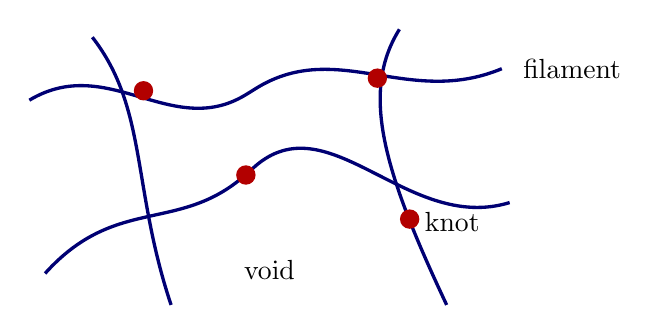
\begin{tikzpicture}[x=1cm,y=1cm]
  \draw[rounded corners=2pt,very thick,blue!45!black]
    (0.2,2.7) .. controls (1.2,3.3) and (2.0,2.2) .. (3.0,2.8)
    .. controls (4.1,3.5) and (5.0,2.6) .. (6.2,3.1);
  \draw[rounded corners=2pt,very thick,blue!45!black]
    (0.4,0.5) .. controls (1.3,1.5) and (2.1,1.0) .. (3.0,1.8)
    .. controls (4.0,2.7) and (5.0,1.0) .. (6.3,1.4);
  \draw[rounded corners=2pt,very thick,blue!45!black]
    (1.0,3.5) .. controls (1.7,2.6) and (1.5,1.6) .. (2.0,0.1);
  \draw[rounded corners=2pt,very thick,blue!45!black]
    (4.9,3.6) .. controls (4.4,2.8) and (4.7,1.8) .. (5.5,0.1);
  \fill[red!70!black] (1.65,2.82) circle (3.5pt);
  \fill[red!70!black] (4.62,2.98) circle (3.5pt);
  \fill[red!70!black] (2.95,1.75) circle (3.5pt);
  \fill[red!70!black] (5.03,1.19) circle (3.5pt);
  \node[align=center] at (3.25,0.55) {void};
  \node[right] at (6.35,3.1) {filament};
  \node[right] at (5.1,1.15) {knot};
\end{tikzpicture}
\caption{Một phép tương tự hai chiều rõ ràng cho mạng caustic: các chỗ tập trung dạng đường bao quanh các khoảng rỗng và gặp nhau tại các nút thắt sáng hơn. Trong ba chiều, các nếp gấp sơ cấp là các tấm mà các giao cắt của chúng tạo thành các sợi và các điểm nút.}
\label{fig:c09-caustic-network}
\end{figure}

Cách dựng không có lực không thay thế cho lý thuyết nhiễu loạn vũ trụ học. Trọng lực là yếu tố then chốt đối với sự tăng trưởng của độ tương phản mật độ, sự hình thành halo, các thiên hà và cấu trúc phi tuyến. Mô hình đồ chơi này tách riêng một sự thật hình học vững chắc: một dòng chảy ban đầu biến thiên nhẹ tự nhiên sẽ gấp nếp và tập trung. Các biến thiên nhỏ của mật độ ban đầu cũng có thể được đưa vào mà không làm thay đổi lập luận Jacobian cốt lõi.

Vì vậy, chúng ta đã dời bí ẩn đi chứ chưa loại bỏ nó. Lạm phát được đưa vào để kéo dãn một vùng cho đến khi nó trở nên cực kỳ phẳng và đồng đều. Phép tính caustic giả định một trường ban đầu gồm những biến thiên vận tốc cực nhỏ. Mầm không đồng nhất đó đến từ đâu? Bài giảng tiếp theo chuyển sang các dao động lượng tử của các trường trong thời kỳ lạm phát và hỏi chúng trở thành các điều kiện ban đầu cho mạng lưới vũ trụ về sau như thế nào.

\section{Những gì lập luận đã xác lập}

Một trường vô hướng đồng nhất ứng xử như một tọa độ chuyển động trong thế năng \(V(\phi)\). Trong một hộp cố định, nó thỏa mãn \(\ddot\phi=-V'(\phi)\). Trong một hộp đồng chuyển động đang giãn nở, thể tích vật lý \(a^3\) xuất hiện trong tác dụng và dẫn đến
\[
\ddot\phi+3H\dot\phi=-V'(\phi).
\]
Ma sát Hubble có thể giữ trường trong một chuyển động tới hạn chậm trên một thế cao và thoải. Khi đó động năng của nó trở nên không đáng kể, thế năng của nó giữ \(H\) gần như không đổi, và \(a(t)\) tăng xấp xỉ theo hàm mũ.

Sự giãn nở làm loãng các đơn cực không mong muốn, làm trơn hình học và đẩy độ cong tiến về 0. Tuy nhiên, lạm phát phải kết thúc. Trường rời khỏi cao nguyên, dao động và truyền năng lượng của nó cho các hạt nóng của giai đoạn nung nóng lại. Một số câu hỏi vẫn còn bỏ ngỏ: dạng của thế năng, bản chất và trạng thái ban đầu của inflaton, các hệ số ghép nung nóng lại của nó, và năng lượng chân không cực nhỏ được quan sát ngày nay.

Thành công của lạm phát đặt ra câu hỏi cuối cùng. Một vũ trụ được làm trơn hoàn hảo sẽ không chứa thiên hà nào. Ánh xạ caustic
\[
y=x+v(x)t,
\qquad
\frac{dn}{dy}=\frac{1}{1+v'(x)t}
\]
cho thấy những biến thiên cực nhỏ trong một dòng chảy ban đầu có thể tạo ra các tấm, các sợi và các nút thắt sắc nét như thế nào. Nó không giải thích nguồn gốc của những biến thiên đó. Nguồn gốc lượng tử của chúng là chủ đề mà lập luận giờ đây chuyển sang.
